\chapter{Warcaby}
\thispagestyle{chapterBeginStyle}
\label{rozdzial1}

Warcaby to jedna z najpopularniejszych klasycznych gier dwuosobowych, zaliczanych do gier z doskonałą informacją i gier o sumie zerowej. Przyjmuje się, że gra ta zrodziła się w XII wieku, najprawdopodobniej na południu Francji lub w Hiszpanii, oraz że wywodzi się ona z dawnej arabskiej gry Alquerque~\cite{Gry}. Istnieją coroczne mistrzostwa i turnieje  światowe w różnych odmianach warcabów, choć dzięki nieskomplikowanym zasadom są one popularne również w mniejszych kręgach.

\section{Reguły warcabów standardowych}

Pojedynczą partię warcabów rozgrywa się na szachownicy 8x8 o polach na zmianę pomalowanych na jasno lub ciemno~(Rys.~\ref{fig:plansza}). W grze wykorzystywane są dwa rodzaje figur - piony i damki. Obydwaj gracze rozstawiają po 12 pionów na ciemnych polach w swoich pierwszych trzech rzędach. Dla rozróżnienia, piony pierwszego gracza są koloru białego, natomiast piony drugiego gracza - czarnego. Celem gry jest wyeliminowanie wszystkich figur przeciwnika lub zablokowanie go, poprzez serię naprzemiennych ruchów swoimi figurami. Zablokowanie gracza oznacza doprowadzenie do takiej sytuacji, w której gracz ten nie jest w stanie wykonać żadnego legalnego ruchu, w momencie gdy następuje jego kolej.

\FloatBarrier

\begin{figure}[h!]
\centering
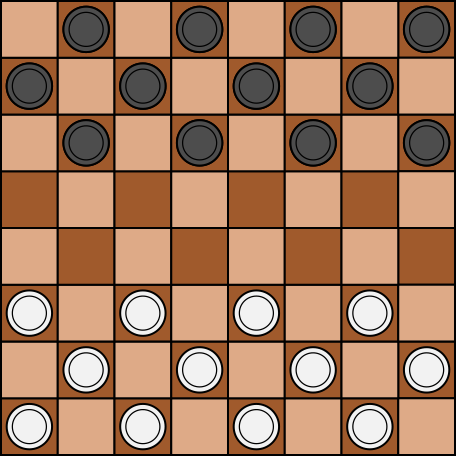
\includegraphics[scale=.6]{graphics/warcaby_planszaStartowa.png}
\caption{Stan początkowy planszy w warcabach.}
\label{fig:plansza}
\end{figure}

\FloatBarrier

Wszystkie figury w grze mogą poruszać się tylko i wyłącznie na ukos (przez co żadne jasne pole na planszy nie zostanie zajęte przez żadną figurę w trakcie rozgrywki). Piony z którymi zaczynają gracze poruszają się tylko o jedno pole w przód względem ich właściciela. Tzn. pion może skoczyć na pole ukośnie sąsiadujące w kierunku oponenta, o ile pole to nie jest zajęte przez inną figurę. W grze istnieje również drugi typ figury - jeżeli pion gracza dojdzie do końca planszy znajdującego się po stronie jego oponenta (do tzw. rzędu awansu), pion zamieniany jest na damkę. Damka jest najpotężniejszą figurą w grze, jako że potrafi poruszać się we wszystkich czterech kierunkach na ukos, a na dodatek przebyć więcej niż jedno pole w linii w jednym ruchu. Pod tym względem damkę najłatwiej porównać z figurą gońca w szachach.

Każdą figurę w warcabach można zbijać, tj. usuwać z obecnej rozgrywki. Piony mogą zbijać sąsiednie figury przeciwnika, wykonując skok nad tą figurą na następne pole w linii prostej, o ile takie pole jest wolne. Piony mogą bić zarówno do przodu, jak i do tyłu. Damki w standardowych warcabach zbijają ze~znacznie większego dystansu (można powiedzieć, że w momencie zbijania ich ,,sąsiadowanie'' z przeciwnymi figurami nie jest ograniczone do jednego pola różnicy). Zbita figura zostaje zdjęta z planszy i nie bierze już udziału w rozgrywce. Nie można bić swoich figur.

Warcaby mają specjalne reguły bicia wyróżniające je spośród innych gier planszowych. Po pierwsze, w jednym ruchu jedna figura może wykonać wiele bić. Jeśli po jednym biciu figura wskoczyła w miejsce, z~którego jest w stanie przeprowadzić kolejne bicie, można takie bicie wykonać w tej samej turze. W~jednym ruchu nie można dwa razy zbić tej samej figury. Po drugie, bicia są obowiązkowe. Jeżeli gracz w~swojej turze jest postawiony w sytuacji, w której co najmniej jedna z jego figur ma możliwość bicia, gracz ten musi wykonać taki ruch. Jeżeli więcej niż jedna figura gracza może wykonać bicie, gracz decyduje którą z tych figur się rusza. Dodatkowo, piony mają większą swobodę w ruchach bijących niż damki. Jeden pion może przeprowadzić dowolny z kilku różnych ruchów bijących, które jest w stanie przeprowadzić. Damki natomiast mają obowiązek maksymalnego bicia, tj. należy wykonać bicie o największej możliwej liczbie zbijanych figur w jednym ruchu.

\section{Wariant angielski}

\FloatBarrier

Praca skupiona jest na szczególnej wersji gry w~warcaby, nazywanej na ogół wariantem angielskim lub w~niektórych kręgach wariantem amerykańskim. Został on wybrany głównie ze~względu na ograniczenie przestrzeni stanów, w~jakich może znaleźć się rozgrywka - reguły gry dostosowane do tego wariantu znacznie zmniejszają liczbę możliwości, które rozgrywający algorytm musi rozpatrzeć.

Wariant ten wprowadza dwie zmiany do zasad gry względem wariantu standardowego (opierając się o~\cite{Gry}). Po pierwsze, piony nie mogą bić do tyłu. Po drugie, damkom ogranicza się możliwość ruchu do~jednego sąsiedniego pola oraz do bicia wyłącznie sąsiadujących przeciwnych figur, lecz wciąż mogą poruszać się we~wszystkich kierunkach na ukos. Jedyną przewagą damek nad pionkami w~tym wariancie jest możliwość ruchu i bicia do tyłu.

\begin{figure}
\centering
\begin{subfigure}{.5\textwidth}
  \centering
  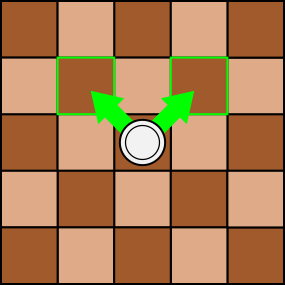
\includegraphics[scale=.6]{graphics/warcaby_ruchyPionZwykle3.png}
  \caption{Legalne ruchy}
  \label{fig:sub1}
\end{subfigure}%
\begin{subfigure}{.5\textwidth}
  \centering
  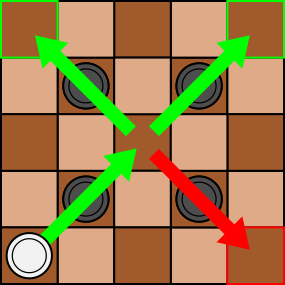
\includegraphics[scale=.6]{graphics/warcaby_ruchyPionBicia.png}
  \caption{Legalne bicia}
  \label{fig:sub2}
\end{subfigure}
\caption{Zestaw możliwych ruchów dla piona w wariancie angielskim}
\label{fig:pion}
\end{figure}

\begin{figure}
\centering
\begin{subfigure}{.5\textwidth}
  \centering
  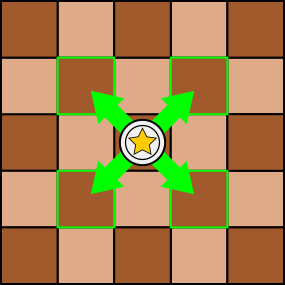
\includegraphics[scale=.6]{graphics/warcaby_ruchyDamkaZwykle.png}
  \caption{Legalne ruchy}
  \label{fig:sub11}
\end{subfigure}%
\begin{subfigure}{.5\textwidth}
  \centering
  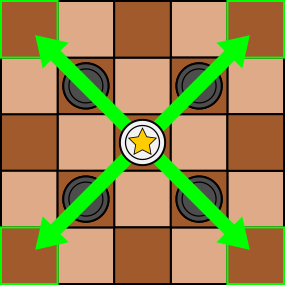
\includegraphics[scale=.6]{graphics/warcaby_ruchyDamkaBicia.png}
  \caption{Legalne bicia}
  \label{fig:sub22}
\end{subfigure}
\caption{Zestaw możliwych ruchów dla damki w wariancie angielskim}
\label{fig:damka}
\end{figure}

\FloatBarrier

Przydatne w implementacji jest rozpatrywanie remisów. W grach towarzyskich remis zazwyczaj następuje za obopólną zgodą graczy. Na arenie turniejowej istnieje parę kryteriów determinujących remis. W~rozpatrywanej wersji wariantu angielskiego wykorzystywana będzie zasada 40 ruchów: rozgrywka kończy się remisem, gdy w 40 naprzemiennych ruchach obu graczy nie została zbita ani jedna figura.

\FloatBarrier

\subsection{Badania wariantu}

Do rozwoju badań nad warcabami w wariancie angielskim najmocniej przyczynił się Jonathan Schaeffer, profesor Uniwersytetu Alberty w Kanadzie. Jego zespół opracował Chinooka, przeszukujący w głąb program do grania w warcaby angielskie, który w roku 1992 oraz 1994 stanął naprzeciw ówczesnego mistrza świata Mariona Tinsleya i ogłoszony został pierwszym komputerowym zwycięzcą mistrzostw~\cite{Chinook}. Następnie, z pomocą programu, udowodnili poprzez słabe rozwiązanie (\textit{weakly solved}, pojęcie omówione w~\cite{Solving}), że każda gra w warcabach angielskich kończy się remisem, pod warunkiem że gracze wykonują ruchy doskonale~\cite{Solved}. Pomimo uproszczonych zasad względem klasycznej wersji, wariant angielski posiada przestrzeń stanów wielkości rzędu $10^{20}$, dlatego też rozwiązanie zajęło zespołowi Schaeffera około 18 lat na 200 równolegle liczących maszynach.



